\chapter{The pn-junction}
\label{ch:pnjunction}

%\section{Chapter Overview}
In this section we demonstrate that when a junction is formed between a sample of $p$-type and one of $n$-type semiconductor, this combination possesses the properties of a rectifier. This two-terminal device is called a \emph{junction diode}. The physical structure and symbol  of a pn-junction is shown in figure \ref{fig:pnjunction}

\begin{figure}[h!]
\centering
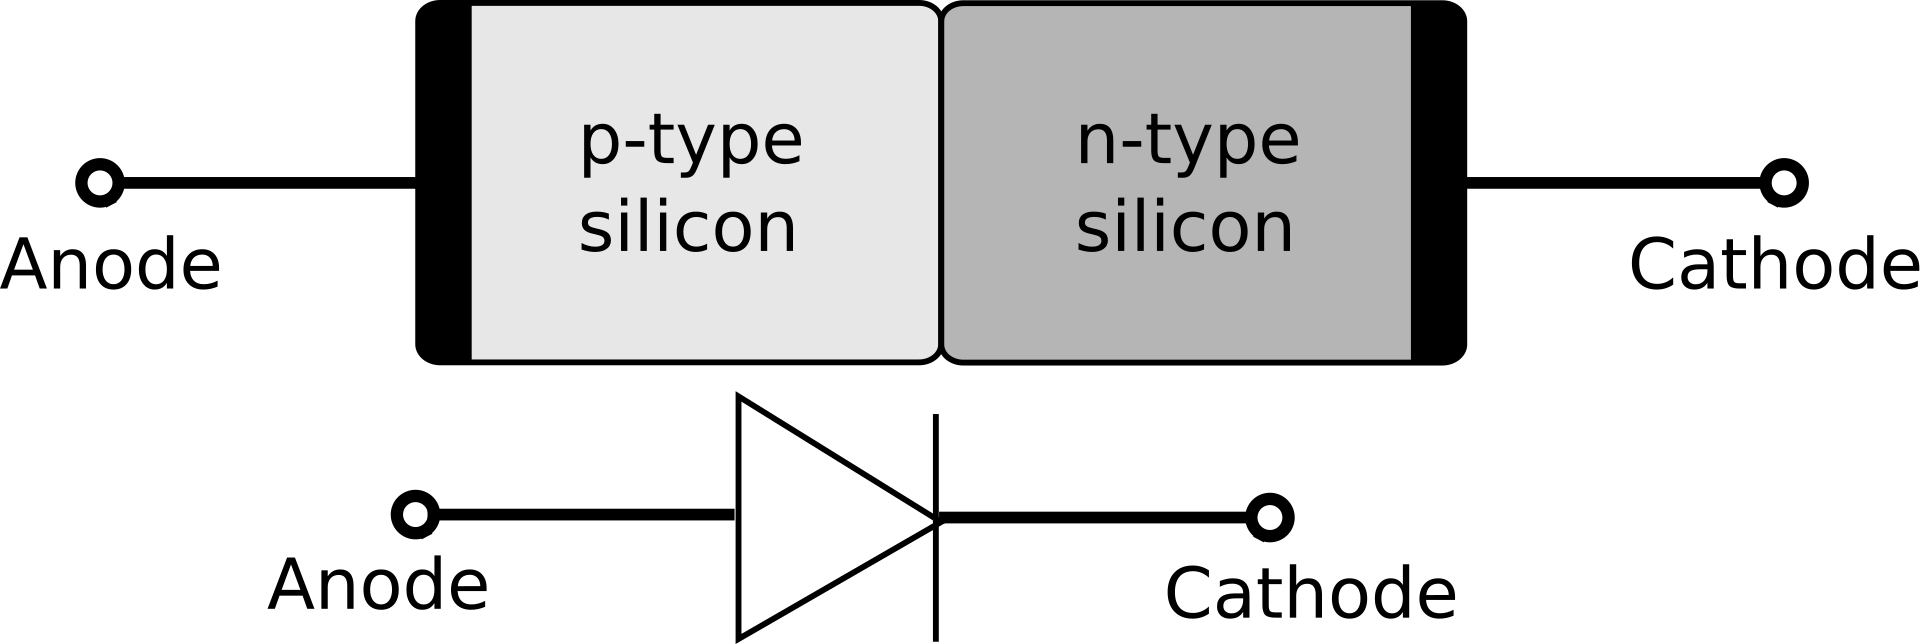
\includegraphics[width=12cm]{figures/ch01/pnjunction.png}
\caption{Structure (above) and symbol (below) of a pn-junction} 
\label{fig:pnjunction}
\end{figure}

We will discuss the junction in equilibrium and under forward and reverse bias. The I-V characteristic will be derived and the concepts of avalanche breakdown and depletion capacitance will be discussed.

\section{The pn-junction in equilibrium}
If donor impurities are introduced into one side and acceptors in the other side of a single crystal of a semiconductor, a $pn$-junction is formed\footnote{This is called an \emph{abrupt junction}}. At the interface, there is by construction a concentration gradient and hence electrons and holes will diffuse to either side. Electrons from the n-type will recombine with the majority holes in the p-type and the holes from the p-type will recombine with the majority electrons in the n-type. As a consequence, the doping ions will be exposed and the n-side will have a fixed positive charge density ($N_d$) while the p-side will have a fixed negative charge density ($N_a$) (figure \ref{fig:pn_equilibrium} (a). This charge buildup will lead to an internal electric field pointing from n-type to p-type and it will thus act against any further diffusion current (\ref{fig:pn_equilibrium} (b)). We assume for now that no external bias is applied, so that no net current can flow. The zone where the majority carriers have diffused and recombined is the \emph{space-charge region}\footnote{Also called the depletion region}. To preserve charge neutrality, we require that:
$$
N_A \; x_p = N_d \; x_n
$$
with $x_p$ and $x_n$ the depth of the space-charge region in p- and n-type ($W_{Dp}$ and $W_{Dn}$ in figure \ref{fig:pn_equilibrium}). As can be deduced from this expression, the space-charge region extends further in the lightly-doped material.\\
Because $\frac{d\mathcal{E}}{dx} = \rho/\epsilon$, the electrical field that results from this charge buildup is computed as $\mathcal{E}(x) = \int \rho(x)/\epsilon \; dx$ with $\rho(x)$ the local charge profile:
\begin{equation}
    \begin{split}
        \rho(x) &= -N_a \text{ if } x < 0 \\
                &= \; N_d \text{ if } x > 0
    \end{split}
\end{equation}
The maximum electric field corresponds to the total charge buildup and is negative since the p-type is placed left: $|\mathcal{E}_m| = \epsilon N_a x_p =  \epsilon N_d x_n$. An electric field gives rise to a potential difference since $\mathcal{E} = -\frac{d\psi}{dx}$ as in figure \ref{fig:pn_equilibrium}(c) where the so-called built-in potential $\psi_{bi}$ is equal to the surface under $\mathcal{E}(x)$:
$$
\psi_{bi} = \frac{1}{2} (x_n + x_p) |\mathcal{E}_m| = \frac{1}{2} \epsilon (x_n + x_p)  N_a x_p
$$
This built-in potential is also visible in \ref{fig:pn_equilibrium} (d) where the energy bands are shown. Due to electric field, the bands will bend (in opposite direction as for the potential, since $E=-qV$) at the junction. This last figure is important and can also be constructed by reasoning with the Fermi levels.\\
The total width $W = x_n + x_p$ of the space charge region can be computed as function of the doping levels and the built-in voltage. The result is:
\begin{equation}
    W = \sqrt{\frac{2 \epsilon}{q} \Big(\frac{N_a + N_d}{N_a N_d}\Big) V_{bi}}
    \label{eq:SCR_width}
\end{equation}

\begin{figure}[h!]
\centering
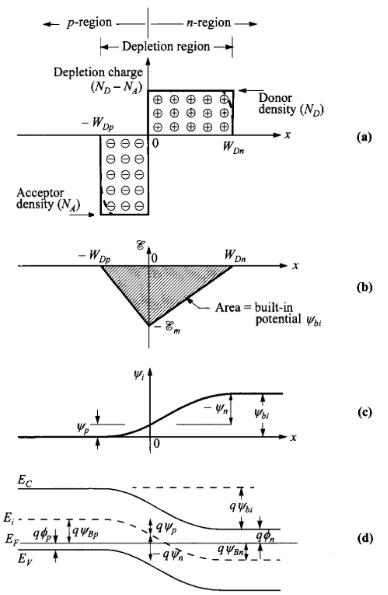
\includegraphics[width=8cm]{figures/ch01/pn_equilibrium.jpg}
\caption{pn-junction in thermal equilibrium} 
\label{fig:pn_equilibrium}
\end{figure}
\subsection{Fermi-levels in equilibrium}
Since no net current can flow in the junction with no external bias, the drift current must be equal to the diffusion current. For the holes, this condition gives:
\begin{equation}
    \begin{split}
       J_p  &= J_{p, drift} + J_{p, diffusion} \\
            &= q \mu_p p \mathcal{E} - q D_p \frac{dp}{dx} \\
            &= q \mu_p p \Big(\frac{1}{q} \frac{dE_i}{dx} \Big) - k T \mu_p \frac{dp}{dx}  = 0\\
    \end{split}
    \label{eq:jp_equilibrium}
\end{equation}
In equilibrium we can apply the Boltzmann equations: 
\begin{equation}
    p = n_i e^{(E_i - E_F)/kT}
    \label{eq:boltzmann_ch2}
\end{equation}
and compute $\frac{dp}{dx}$:
$$
\frac{dp}{dx} = \frac{p}{kT} \Big( \frac{dE_i}{dx} - \frac{dE_F}{dx} \Big)
$$
Substituting this in equation \ref{eq:jp_equilibrium} gives:
$$
J_p = \mu_p p \frac{dE_F}{dx} = 0 
$$
or $\frac{dE_F}{dx} = 0$. A similar result is valid for the electrons. \textbf{For there to be zero net electron and hole currents, the Fermi level must be constant.}\\
As can be seen in figure \ref{fig:pn_equilibrium}(d), the Fermi level $E_F$ remains constant along the junction because there is no net current. Since $E_F$ is close to $E_V$ in the p-type and close the $E_C$ in the n-type, the bands must bend like they do  in the figure to keep a constant $E_F$.

\subsection{The built-in potential}
We will now compute $V_{bi} = \psi_n - \psi_p$ (previously denoted as $\psi_{bi}$). We know that far away from the junction, no net charges are present, so the potential must comply with the Laplace equation:
$$
\frac{d^2 \psi}{dx^2} = 0
$$
and $N_d - N_a + p - n = 0$ to preserve charge neutrality. In a p-type material, we assume that $N_d = 0$ and $p \gg n$. This results in $p = N_a$. Inserting this in equation \ref{eq:boltzmann_ch2} gives:
$$
\psi_p = -\frac{1}{q} (E_i - E_f) |_{x < x_p} = \frac{kT}{q} \ln\Big(\frac{N_a}{n_i}\Big)
$$
Similarly, the electrostatic potential for the n-type material is
$$
\psi_n = -\frac{1}{q} (E_i - E_f) |_{x > x_n} = \frac{kT}{q} \ln\Big(\frac{N_d}{n_i}\Big)
$$
The built-in potential $V_{bi}$ is the difference of electrostatic potential between p-side and n-side at thermal equilibrium:
\begin{equation}
    V_{bi} = \psi_n - \psi_p = \frac{kT}{q} \ln\Big(\frac{N_a N_d}{n_i^2}\Big)
    \label{eq:vbi}
\end{equation}

\section{The pn-junction under bias}

\subsection{Forward bias}
Assume we apply a positive voltage $V_F$ to the anode (p-side) while keeping the cathode (n-side) at ground. The effect is that we reduce the barrier of the built-in potential from $V_{bi}$ to $V_{bi} - V_F$, as shown on the left side of figure \ref{fig:pn_bias}. This has a couple of consequences:
\begin{itemize}
    \item The width of the depletion region will reduce, because equation \ref{eq:SCR_width} can be rewritten as:
    \begin{equation}
        W = \sqrt{\frac{2 \epsilon}{q} \Big(\frac{N_a + N_d}{N_a N_d}\Big) (V_{bi} - V_F)}
        \label{eq:SCR_width_bias}
    \end{equation}
    \item The value of the maximum $\mathcal{E}$ is reduced. This means that there is an disequilibrium between diffusion and drift current, and there will be a net (diffusion) flow of holes from p-type to n-type and a flow of electrons from n-side to p-side. The result is a net current from p-side to n-side.\footnote{Notice that electrons can diffuse from low to higher energy, while they always drift from high to low.}
\end{itemize}
There is thus a diffusion current of majority carriers through the depletion region to the other side, where they become the minority carriers. Since there are a lot of majority carriers available, this current can become very large when the potential barrier is lowered enough.\\
Also notice that the Fermi levels in figure \ref{fig:pn_bias} are no longer constant, because there is a current and we are no longer in equilibrium.

\begin{figure}[h!]
\centering
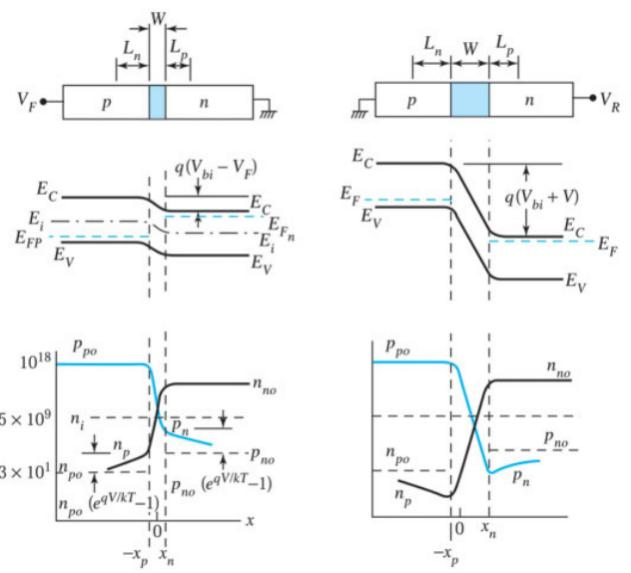
\includegraphics[width=12cm]{figures/ch01/pn_bias.jpg}
\caption{pn-junction under forward (left) and reverse (right) bias} 
\label{fig:pn_bias}
\end{figure}

\subsection{Reverse Bias}
When we apply a positive voltage $V_R$ to the cathode (n-side) while keeping the anode at ground, we increase the barrier of the built-in potential to $V_{bi} + V_R$. This situation is sketched on the right of figure \ref{fig:pn_bias}. According to equation \ref{eq:SCR_width_bias}, the width of the space-charge region will increase (because we can replace $V_F$ with $-V_R$). The internal electric field at the junction becomes larger than before, so there can be a net drift current. However, the only available carriers to be swept across the space-charge region by the electric field are the minority carriers on both sides of the junction. Consequently, the resulting current (the \emph{saturation current}) will be very low.

\subsection{Diode Characteristic}
Let's to compute the currents. We'll make the following assumptions:
\begin{enumerate}
    \item the depletion region has abrupt boundaries and, outside the boundaries, the semiconductor is assumed to be neutral; 
    \item the carrier densities at the boundaries are related by the electrostatic potential difference across the junction; 
    \item the injected minority carrier densities are small compared to the majority carrier densities;
    \item neither generation nor recombination current exists in the depletion region and the electron and hole currents are constant throughout the depletion region.
\end{enumerate}
At equilibrium, we get $p_{p0} = N_a$ and $n_{n0} = N_d$. Together with the mass-action law $p_{p0} \; n_{n0} = n_i^2$, we can rewrite equation \ref{eq:vbi} as:
$$
V_{bi} = \frac{kT}{q} \ln \frac{p_{p0} n_{n0}}{n_i^2} = \frac{kT}{q} \ln \frac{n_{n0}}{n_{p0}}
$$
Rearranging this gives:
\begin{equation}
    \begin{split}
        n_{n0} &= n_{p0} e^{qV_{bi}/kT}
    \end{split}
    \label{eq:nn0}
\end{equation}
and
\begin{equation}
	\begin{split}
		p_{p0} &= p_{n0} e^{qV_{bi}/kT}
	\end{split}
	\label{eq:pp0}
\end{equation}
Because of the second assumption, these equations remain valid when we change the net potential. Thus:
\begin{equation}
    \begin{split}
        n_{n} &= n_{p} e^{q(V_{bi}-V_F)/kT}
    \end{split}
    \label{eq:nn}
\end{equation}
with $n_n$ and $n_p$ the non-equilibrium electron densities at the boundaries of the space-charge region at n- and p-sides, respectively. Substituting \ref{eq:nn0} in \ref{eq:nn} yields the electron density at the boundary of the depletion region on the p-side ($x = –x_p$): 
\begin{equation}
	n_p = n_{p0}\;e^{qV/kT}
\end{equation}
and similarly:
\begin{equation}
	p_n = p_{n0}\;e^{qV/kT}
	\label{eq:density_junction}
\end{equation}
where $V$ can be both $V_F$ or $V_R$, namely the externally applied voltage across the junction. We can also write this as:
\begin{equation}
	\begin{split}
		n_p - n_{p0} &= n_{p0}(e^{qV/kT} - 1) \\
		p_n - p_{n0} &= p_{0}(e^{qV/kT} - 1)
	\end{split}
\label{eq:pexcess_depletion}
\end{equation}
Note that the minority carriers at the boundaries of the space-charge region increase substantially above their equilibrium under forward bias. Hence, there is an injection of minority carriers at the depletion region.\\
In the neutral n-region, there is no electric field, so the steady-state continuity equation \ref{eq:continuity} reduces to:
\begin{equation}
\frac{\partial p_n}{\partial t} = D_p \frac{d^2p}{dx^2} - \frac{p_n - p_{n0}}{\tau_p} = 0
\end{equation} 
Solving this equation with boundary conditions of eq. \ref{eq:pexcess_depletion} and $p_n(x = \infty) = p_{n0}$ gives:

\begin{equation}
p_n - p_{n0} =  p_{n0} (e^{qV/kT} - 1) e^{-(x-x_n)/L_p}
\end{equation} 
with $L_p = \sqrt{D_p \tau_p}$ the diffusion length of holes. This graph is shown in the lower left part of figure \ref{fig:pn_bias}. At the boundary $x=x_n$:

\begin{equation}
J_p(x_n) = -qD_p \frac{dp_n}{dx}\Bigg|_{x=x_n} = \frac{qD_pp_{n0}}{L_p}(e^{qV/kT} - 1)
\end{equation} 

By applying the same reasoning for the n-region, we obtain a similar relation for $J_n$. Since the total current is the sum of both, we finally find:
\begin{equation}
J = J_p(x_n) + J_n(-x_p) = J_S(e^{qV/kT} - 1)
\label{eq:ideal_diode}
\end{equation} 
with $J_S$ the saturation current:
\begin{equation}
J_S = \frac{qD_n p_{n0}}{L_p} + \frac{D_n n_{p0}}{L_n}
\end{equation} 
Equation \ref{eq:ideal_diode} is the diode equation. Its graph is shown in figure \ref{fig:diode_charac}. It is important to notice that the current increases exponentially when $V>0$ because the potential barrier is removed. The junction will act as a conductor. On the other hand, when $V<0$, there is only a small saturation current that is not impacted by the value of $V$. The junction is an open circuit (with a loss current).

\begin{figure}[h!]
\centering
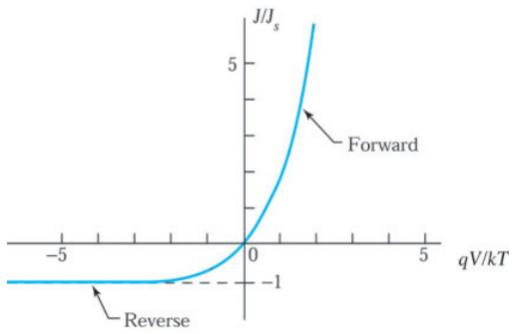
\includegraphics[width=8cm]{figures/ch01/diode_charac.jpg}
\caption{Current characteristic of equation \ref{eq:ideal_diode}}
\label{fig:diode_charac}
\end{figure}

\subsection{Practical Diode Characteristic}
Equation \ref{eq:ideal_diode} gives a current density. By multiplying with the surface $A$ of the cross-section of the junction, we obtain the I-V curve:
\begin{equation}
i_D = I_S(e^{v_D/v_{th}} - 1)
\label{eq:idiode_IV}
\end{equation} 
with $v_{th} = \frac{kT}{q} \approx 26 mV$ (at $T=300K$) the thermal voltage (see figure \ref{fig:diode_charac2}). When $v_D \gg v_{th}$:
\begin{equation}
i_D \approx I_S e^{v_D/v_{th}}
\end{equation} 
Furthermore, as $v_D$ increases by $\sim 60 mV$, the current $i_D$ is multiplied by a factor 10. As can be seen in figure \ref{fig:diode_charac2}, we can consider $v_D = 0.6V$ as a threshold voltage:
\begin{itemize}
    \item If $v_D > 0.6V$, the diode will conduct,
    \item If $v_D < 0.6V$, the diode will not conduct.
\end{itemize}
Hence the diode works as a rectifier: only current from p- to n-side can pass, while the other direction is blocked. Off course, because of the saturation current and the avalanche effect (see \ref{sec:avalanche}) this is not completely true.

\begin{figure}[h!]
\centering
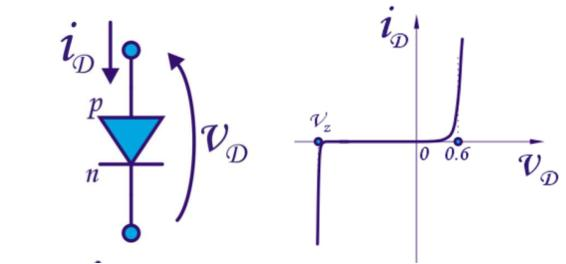
\includegraphics[width=12cm]{figures/ch01/diode_charac2.jpg}
\caption{Symbol and I-V curve} 
\label{fig:diode_charac2}
\end{figure}

\section{Tunnel \& Avalanche effect}
\label{sec:avalanche}
From figure \ref{fig:diode_charac2}, we see that there is also a point where the diode will conduct under reverse bias. This phenomenom can have two causes: either we speak of junction breakdown due to the avalanche effect, or Zener breakdwon, due to the tunnel effect. Junction breakdown happens at high voltages and is typically unwanted. Zener breakdown can be useful and the doping is adapted such that it occurs at a couple of volts. It is for example used in voltage references (see chapter \ref{ch:references}).\\
\begin{minipage}{.5\textwidth}
	\centering
	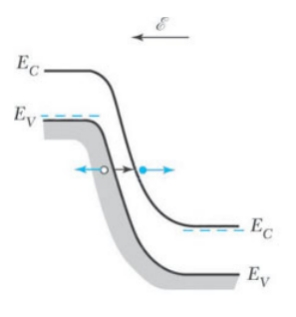
\includegraphics[height=6cm]{figures/ch01/tunnel_effect.jpg}
	\captionof{figure}{}
	\label{fig:tunnel_effect}
\end{minipage}
\begin{minipage}{.5\textwidth}
	\centering
	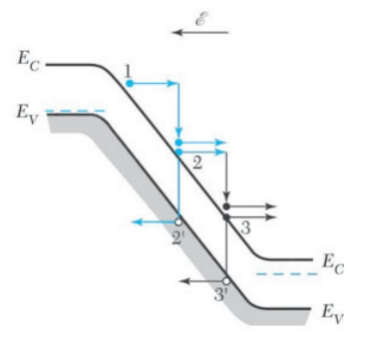
\includegraphics[width=6cm]{figures/ch01/avalanche.jpg}
	\captionof{figure}{}
	\label{fig:avalanche}
\end{minipage}\\
The \emph{tunnel effect} relies on quantum tunneling: when a high electric field is applied to a p–n junction in the reverse direction, as in figure \ref{fig:tunnel_effect}, the distance between valence and conduction band becomes locally very narrow. Under these circumstances, a valence electron can make a transition from the valence band to the conduction band. This process, in which an electron penetrates through the energy bandgap, is called tunneling. The resulting electron and hole is then swept by the electric field through the space-charge region, which creates a Zener current.\\
We speak of the \emph{avalanche effect} when a thermally generated electron in the space-charge region (designated by $1$ in figure \ref{fig:avalanche}) gains kinetic energy from the electric field. If the field is sufficiently high, the electron can gain enough kinetic energy that on collision with an atom, it can break the lattice bonds, creating an electron-hole pair ($2$ and $2'$). The newly created electron and hole both acquire kinetic energy from the field and create additional electron-hole pairs (e.g., $3$ and $3'$). These in turn continue the process, creating other electron-hole pairs. This process is therefore called avalanche multiplication.

\section{Depletion Capacitance}
\label{sec:depletion_capacitance}
When we reverse-bias a pn-junction, more positive charges appear on the n-side and more negative charges on the p-side. Thus, the device basically operates as a \emph{capacitor}. In essence, we can view the conductive $n$ and $p$ sections as the two plates of the capacitor. We also assume the charge in the depletion region equivalently resides on each plate.\\
But there is more: as $V_R$ increases, so does the width of the depletion region. That is, the capacitance of the structure decreases as the two plates move away from each other. The junction therefore displays a voltage-dependent capacitance. We can show that the junction capacitance $C_j$ is given by:
\begin{equation}
	C_j = \frac{C_{j0}}{\sqrt{1 - \frac{V_R}{V_{bi}}}}
\end{equation}
with $C_{j0}$ the capacitance under zero external bias ($V_R = 0$).\\
A pn-junction under reverse bias is thus a voltage-controllable capacitor. This kind of device has many uses, like e.g. in frequency-tunable circuits.

\section{Photodetector}
When we reverse-bias a pn-junction made of a direct-bandgap semiconductor like GaAs, we make a photodetector, as in figure \ref{fig:photodetector}. If a photon impinges on an electron in a covalent bond, it can break this bond if the energy $h \nu$ is higher than the bandgap energy. The resulting electron-hole pair is then swept across the space-charge region by the applied electric field. They recombine in the neutral zones, generating a current proportional to the number of photons that impinge on the junction.

\begin{figure}[h!]
	\centering
	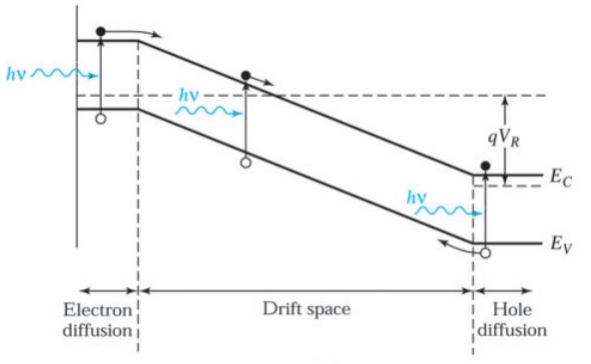
\includegraphics[width=10cm]{figures/ch01/photodetector.jpg}
	\caption{Photodetector operation} 
	\label{fig:photodetector}
\end{figure}
